\documentclass{article}
\usepackage[paperwidth=360pt,paperheight=245pt,margin=0pt,noheadfoot]{geometry}
\usepackage{tikz}
\usetikzlibrary{calc}

\definecolor{ink}{RGB}{28,41,56}
\definecolor{axis}{RGB}{100,116,139}
\definecolor{grid}{RGB}{203,213,225}
\definecolor{curve}{RGB}{30,64,175}
\definecolor{teal}{RGB}{13,148,136}
\definecolor{tealfill}{RGB}{176,227,219}
% Integral diagrams use exactly one semantic palette: blue for the
% lower-only part, yellow for the upper-only (or still unresolved) part, and
% green for their common part.  The common part is explicit rather than an
% alpha blend, so the three meanings stay distinct after GIF quantization.
\definecolor{blue}{RGB}{0,114,178}
\definecolor{bluefill}{RGB}{86,180,233}
\definecolor{yellow}{RGB}{230,159,0}
\definecolor{yellowfill}{RGB}{255,218,102}
\definecolor{green}{RGB}{0,128,84}
\definecolor{greenfill}{RGB}{89,190,142}
\definecolor{orange}{RGB}{234,88,12}
\definecolor{orangefill}{RGB}{254,215,170}
\definecolor{purple}{RGB}{126,34,206}
\definecolor{yellowedge}{RGB}{202,138,4}
\definecolor{projection}{RGB}{148,163,184}
\colorlet{under}{blue}
\colorlet{underfill}{bluefill}
\colorlet{over}{yellow}
\colorlet{overfill}{yellowfill}
\colorlet{shared}{green}
\colorlet{sharedfill}{greenfill}
\colorlet{gap}{yellow}
\colorlet{gapfill}{yellowfill}

\pagestyle{empty}
\setlength\parindent{0pt}
\setlength\topskip{0pt}
\begin{document}
\noindent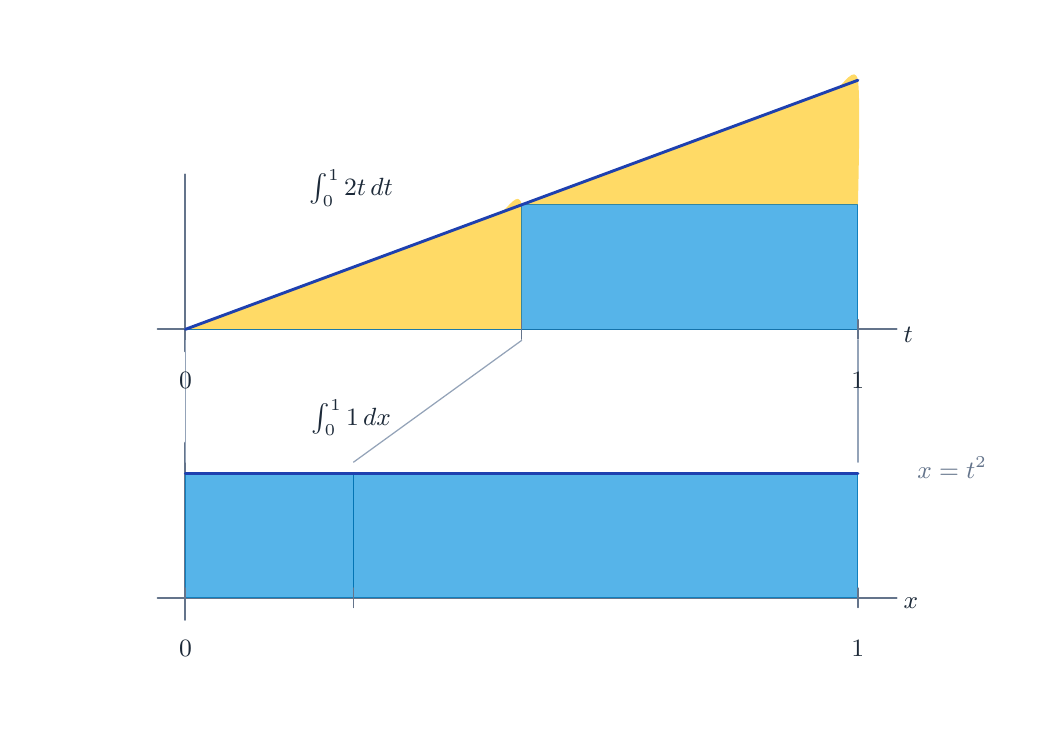
\begin{tikzpicture}[baseline=(current bounding box.north),x=1pt,y=1pt,line cap=round,line join=round]
\useasboundingbox (0,0) rectangle (360,245);
\draw[axis,line width=.75pt] (47,136) -- (314,136);
\draw[axis,line width=.75pt] (57,128) -- (57,192);
\draw[axis,line width=.75pt] (47,39) -- (314,39);
\draw[axis,line width=.75pt] (57,31) -- (57,95);
\path[fill=gapfill] plot[smooth] coordinates {(57,136) (57,136) (64.5938,138.8125) (72.1875,141.625) (79.7812,144.4375) (87.375,147.25) (94.9688,150.0625) (102.5625,152.875) (110.1562,155.6875) (117.75,158.5) (125.3438,161.3125) (132.9375,164.125) (140.5312,166.9375) (148.125,169.75) (155.7188,172.5625) (163.3125,175.375) (170.9062,178.1875) (178.5,181) (178.5,136)} -- cycle;
\path[fill=underfill,draw=under,draw opacity=.8,line width=.4pt] (57,136) rectangle (178.5,136);
\path[fill=underfill,draw=under,draw opacity=.8,line width=.4pt] (57,39) rectangle (117.75,84);
\path[fill=gapfill] plot[smooth] coordinates {(178.5,181) (178.5,181) (186.0938,183.8125) (193.6875,186.625) (201.2812,189.4375) (208.875,192.25) (216.4688,195.0625) (224.0625,197.875) (231.6562,200.6875) (239.25,203.5) (246.8438,206.3125) (254.4375,209.125) (262.0312,211.9375) (269.625,214.75) (277.2188,217.5625) (284.8125,220.375) (292.4062,223.1875) (300,226) (300,181)} -- cycle;
\path[fill=underfill,draw=under,draw opacity=.8,line width=.4pt] (178.5,136) rectangle (300,181);
\path[fill=underfill,draw=under,draw opacity=.8,line width=.4pt] (117.75,39) rectangle (300,84);
\draw[projection,line width=.45pt] (57,132) -- (57,88);
\draw[axis,line width=.55pt] (57,132.5) -- (57,139.5);
\draw[axis,line width=.55pt] (57,35.5) -- (57,42.5);
\draw[projection,line width=.45pt] (178.5,132) -- (117.75,88);
\draw[axis,line width=.55pt] (178.5,132.5) -- (178.5,139.5);
\draw[axis,line width=.55pt] (117.75,35.5) -- (117.75,42.5);
\draw[projection,line width=.45pt] (300,132) -- (300,88);
\draw[axis,line width=.55pt] (300,132.5) -- (300,139.5);
\draw[axis,line width=.55pt] (300,35.5) -- (300,42.5);
\draw[curve,line width=1.05pt] plot[smooth] coordinates {(57,136) (60.0375,137.125) (63.075,138.25) (66.1125,139.375) (69.15,140.5) (72.1875,141.625) (75.225,142.75) (78.2625,143.875) (81.3,145) (84.3375,146.125) (87.375,147.25) (90.4125,148.375) (93.45,149.5) (96.4875,150.625) (99.525,151.75) (102.5625,152.875) (105.6,154) (108.6375,155.125) (111.675,156.25) (114.7125,157.375) (117.75,158.5) (120.7875,159.625) (123.825,160.75) (126.8625,161.875) (129.9,163) (132.9375,164.125) (135.975,165.25) (139.0125,166.375) (142.05,167.5) (145.0875,168.625) (148.125,169.75) (151.1625,170.875) (154.2,172) (157.2375,173.125) (160.275,174.25) (163.3125,175.375) (166.35,176.5) (169.3875,177.625) (172.425,178.75) (175.4625,179.875) (178.5,181) (181.5375,182.125) (184.575,183.25) (187.6125,184.375) (190.65,185.5) (193.6875,186.625) (196.725,187.75) (199.7625,188.875) (202.8,190) (205.8375,191.125) (208.875,192.25) (211.9125,193.375) (214.95,194.5) (217.9875,195.625) (221.025,196.75) (224.0625,197.875) (227.1,199) (230.1375,200.125) (233.175,201.25) (236.2125,202.375) (239.25,203.5) (242.2875,204.625) (245.325,205.75) (248.3625,206.875) (251.4,208) (254.4375,209.125) (257.475,210.25) (260.5125,211.375) (263.55,212.5) (266.5875,213.625) (269.625,214.75) (272.6625,215.875) (275.7,217) (278.7375,218.125) (281.775,219.25) (284.8125,220.375) (287.85,221.5) (290.8875,222.625) (293.925,223.75) (296.9625,224.875) (300,226)};
\draw[curve,line width=1.05pt] (57,84) -- (300,84);
\node[font=\small,text=ink,anchor=north] at (57,124) {$0$};
\node[font=\small,text=ink,anchor=north] at (300,124) {$1$};
\node[font=\small,text=ink,anchor=north] at (57,27) {$0$};
\node[font=\small,text=ink,anchor=north] at (300,27) {$1$};
\node[font=\small,text=ink,anchor=west] at (313,134) {$t$};
\node[font=\small,text=ink,anchor=west] at (313,37) {$x$};
\node[font=\small,text=ink,anchor=south] at (117,177) {$\int_0^1 2t\,dt$};
\node[font=\small,text=ink,anchor=south] at (117,94) {$\int_0^1 1\,dx$};
\node[font=\small,text=ink,anchor=west,text=axis] at (318,86) {$x=t^2$};
\end{tikzpicture}
\end{document}
